\begin{frame}
  \frametitle{V\&V Study 2: MSRE Pump Start-up \& Coast-Down Transients}
  This study is based on two transient flow-rate tests on the MSRE under zero-power conditions.
  Starting from zero power critical states with/without forced flow, the fuel salt pump was coasted
  down/started up.
  \pause
  \begin{columns}
    \column[t]{5.5cm}
    \begin{figure}
      \centering
      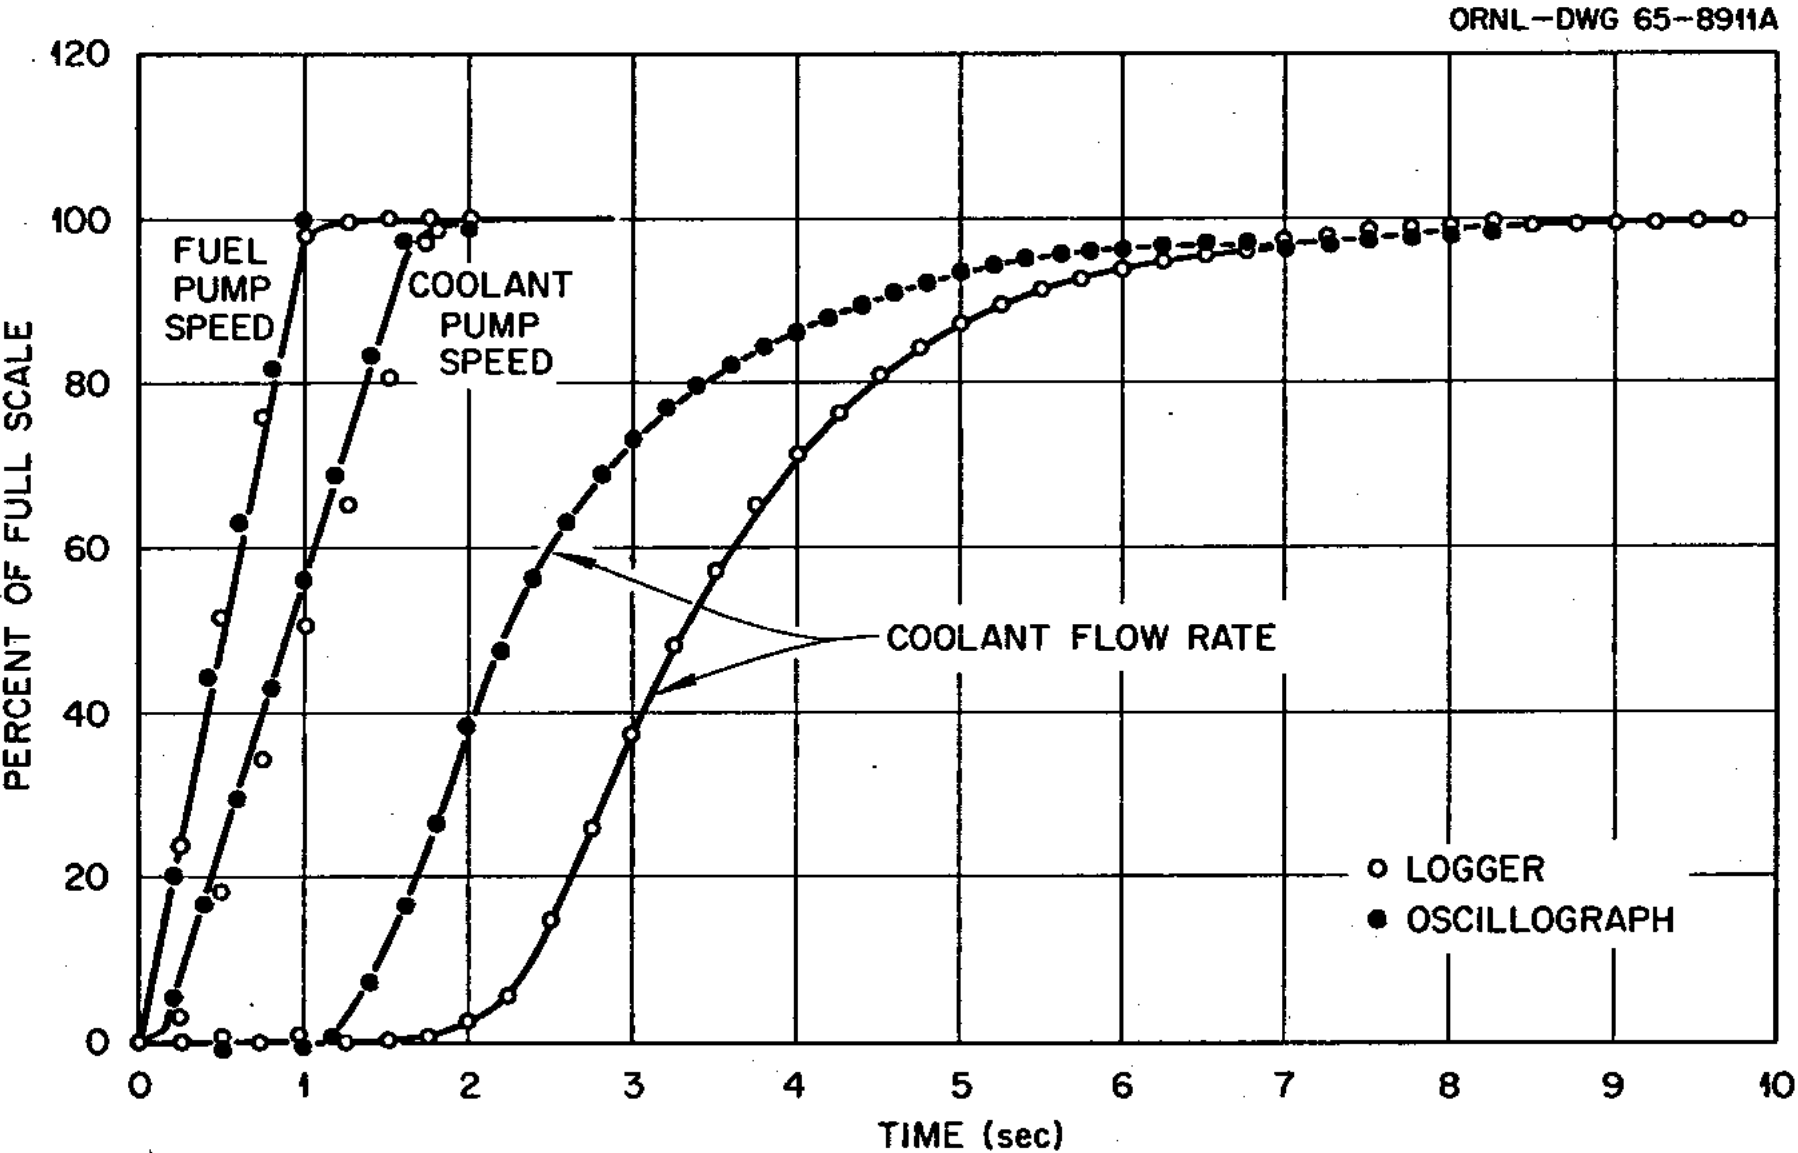
\includegraphics[width=.8\columnwidth]{images/msre-startup}
      \caption{Start-up pump speed and flow rate \cite{prince_zero-power_1968}.}
    \end{figure}
    \column[t]{5.5cm}
    \begin{figure}
      \centering
      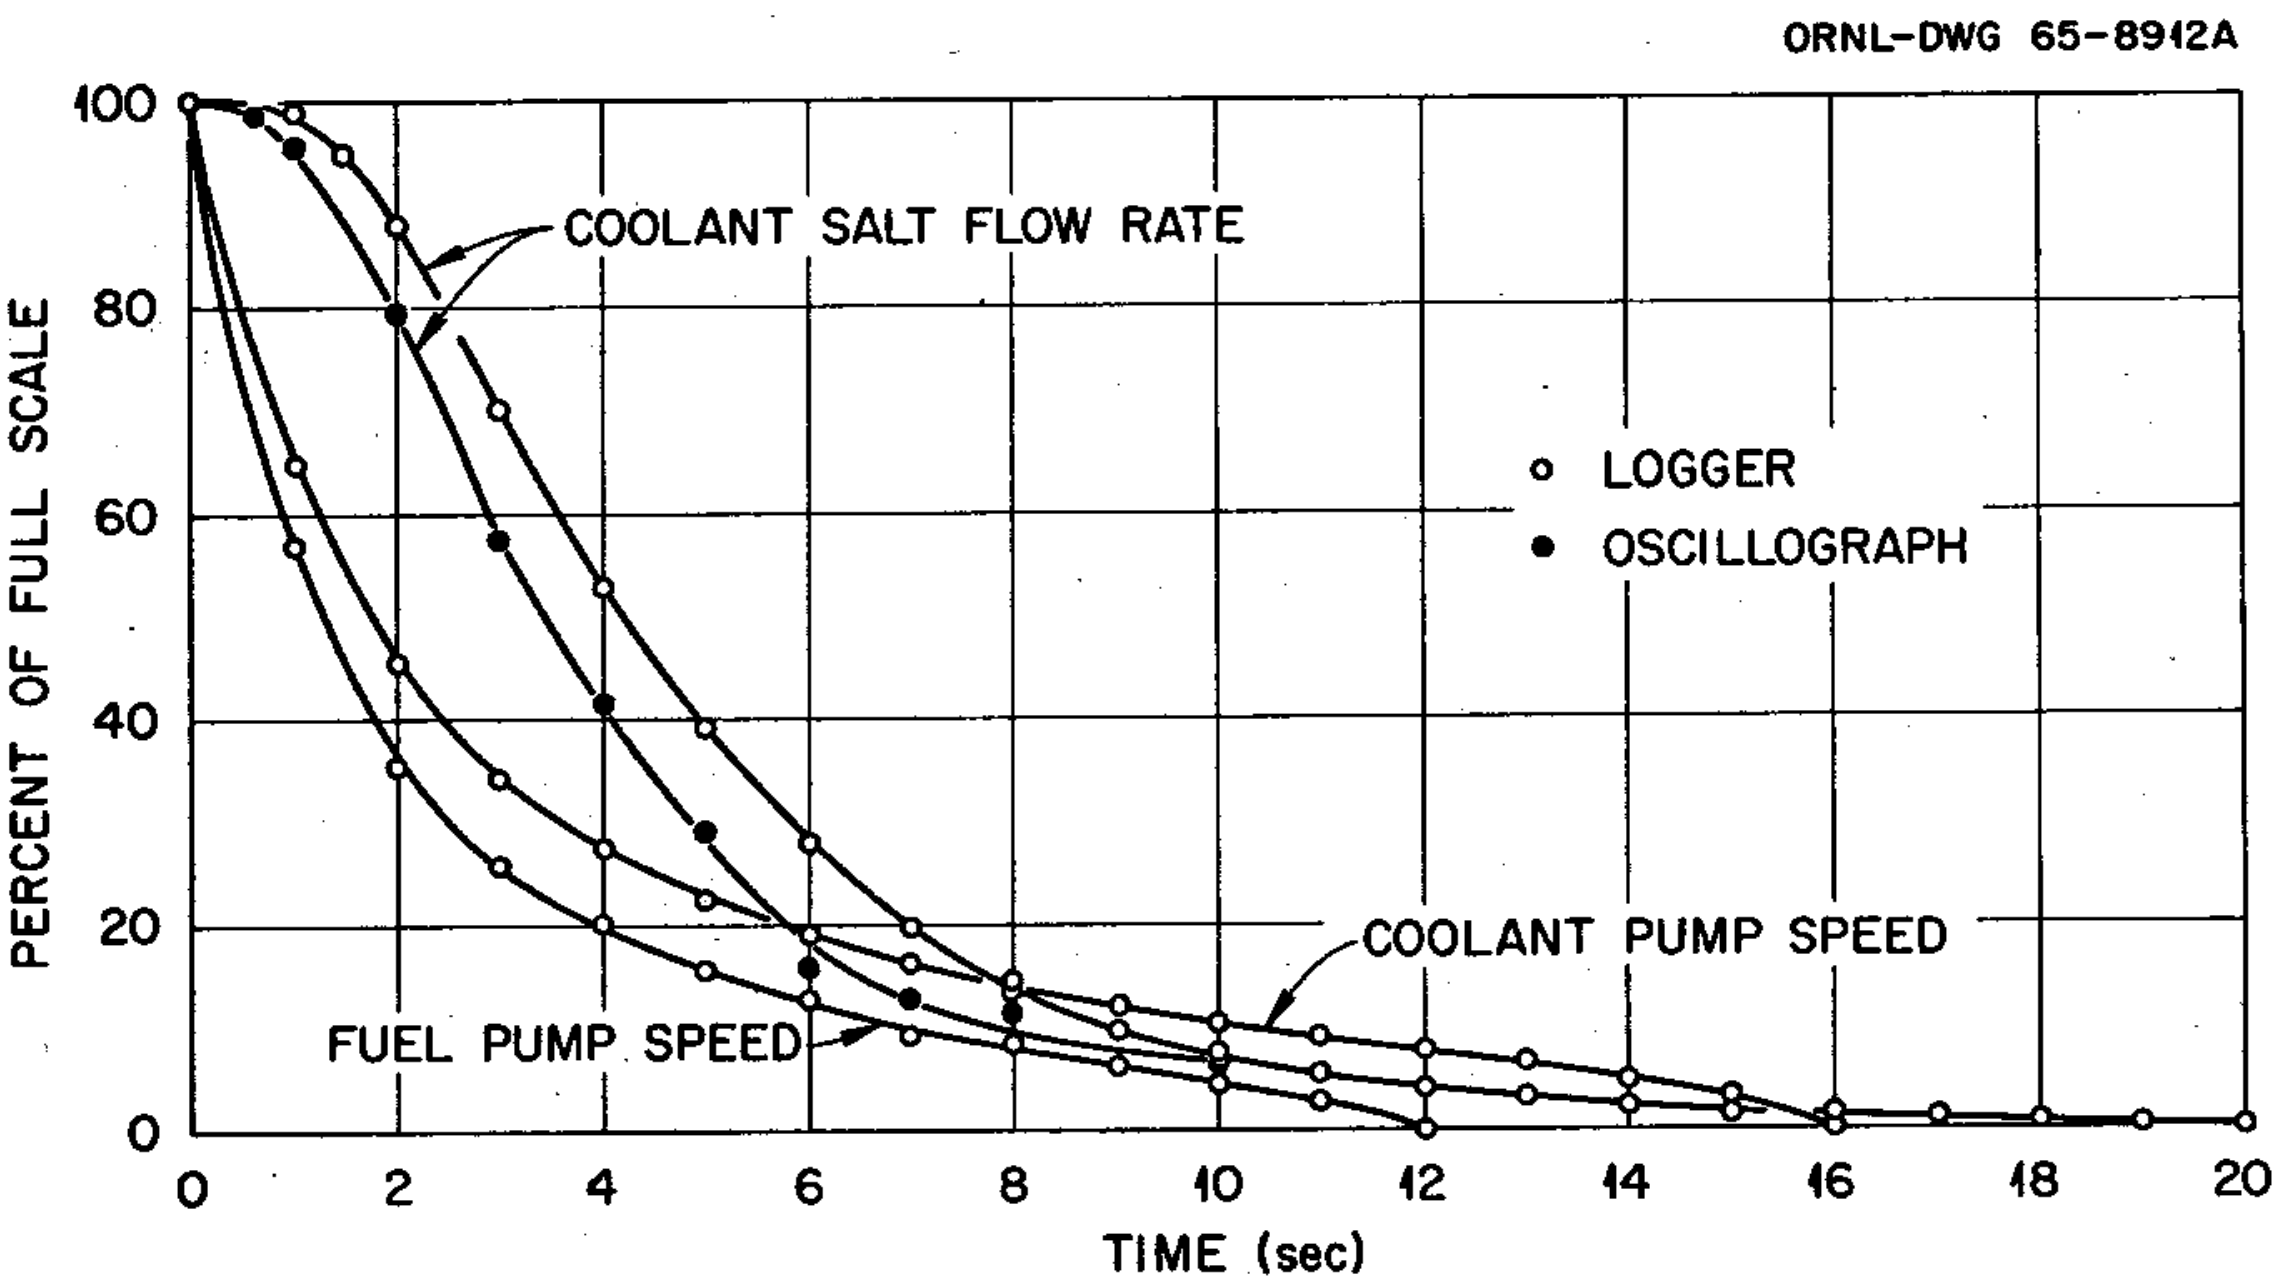
\includegraphics[width=.95\columnwidth]{images/msre-coastdown}
      \caption{Coast-down pump speed and flow rate \cite{prince_zero-power_1968}.}
    \end{figure}
  \end{columns}
\end{frame}

\begin{frame}
  \frametitle{V\&V Study 2: MSRE Pump Start-up \& Coast-Down Transients}
  \begin{columns}
    \column[t]{4cm}
    \begin{figure}
      \centering
      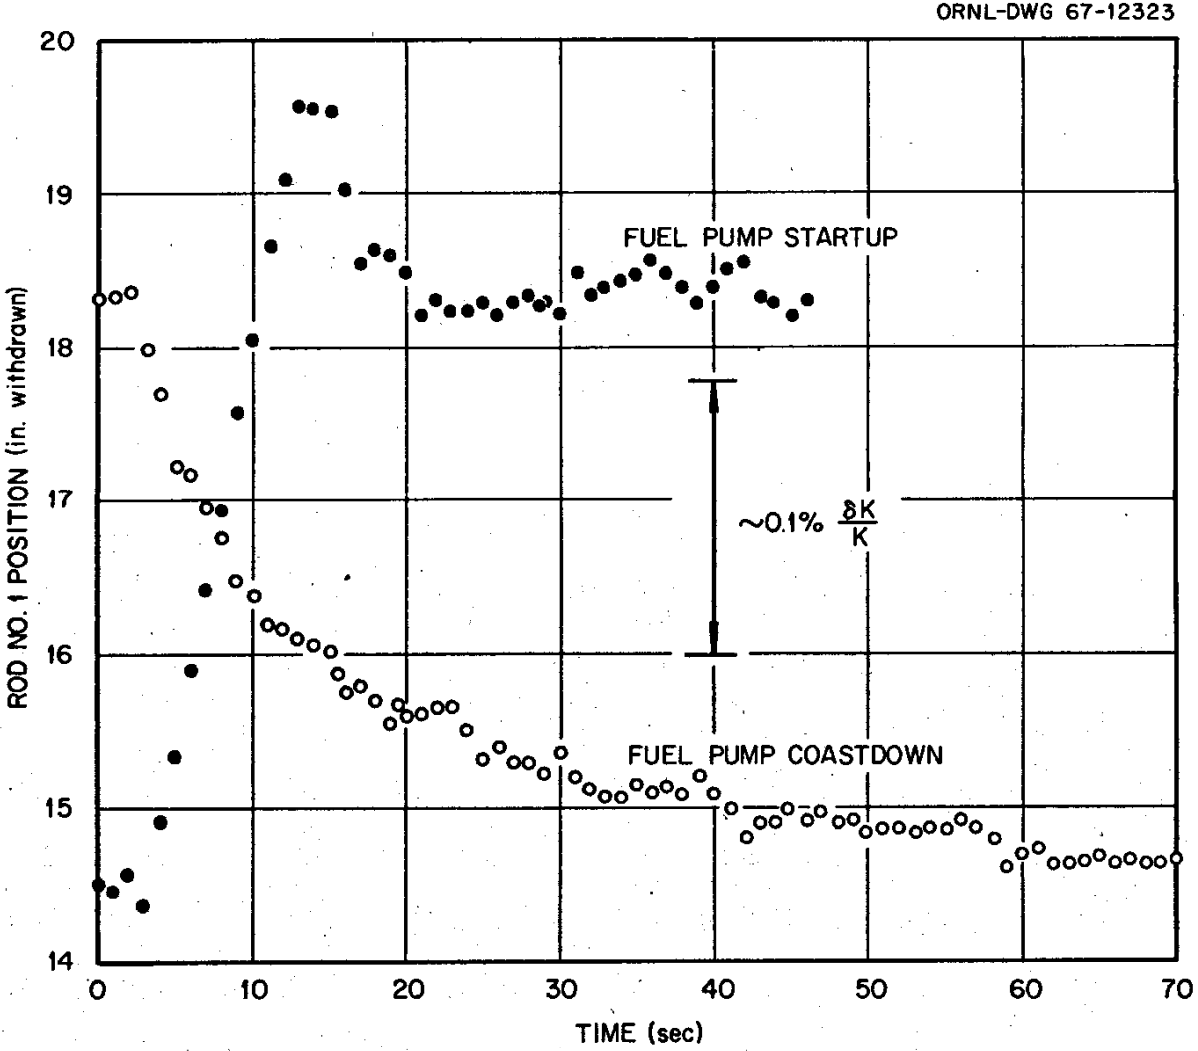
\includegraphics[width=.9\columnwidth]{../images/msre-transient}
      \caption{Control rod response to fuel pump start-up and coast-down
      \cite{prince_zero-power_1968}.}
    \end{figure}
    \hfill
    \column[t]{4cm}
    \begin{figure}
      \centering
      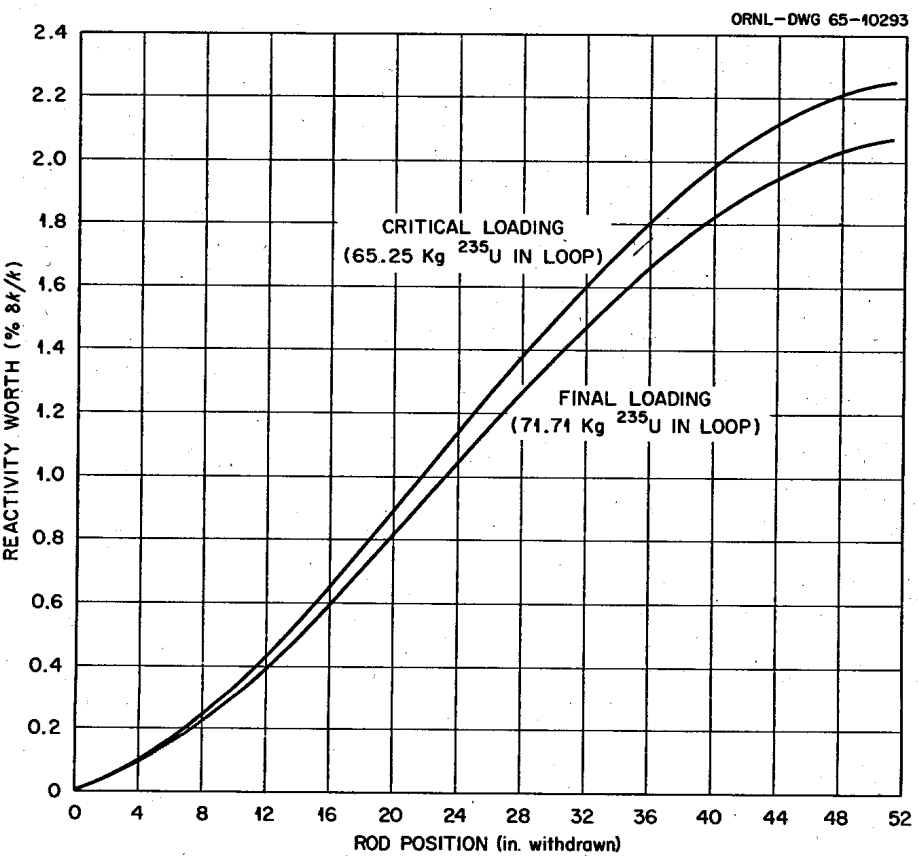
\includegraphics[width=.9\columnwidth]{../images/msre-rod-worth}
      \caption{Integral rod worth \cite{prince_zero-power_1968}.}
    \end{figure}
    \hfill
    \column[t]{4cm}
    \begin{figure}
      \centering
      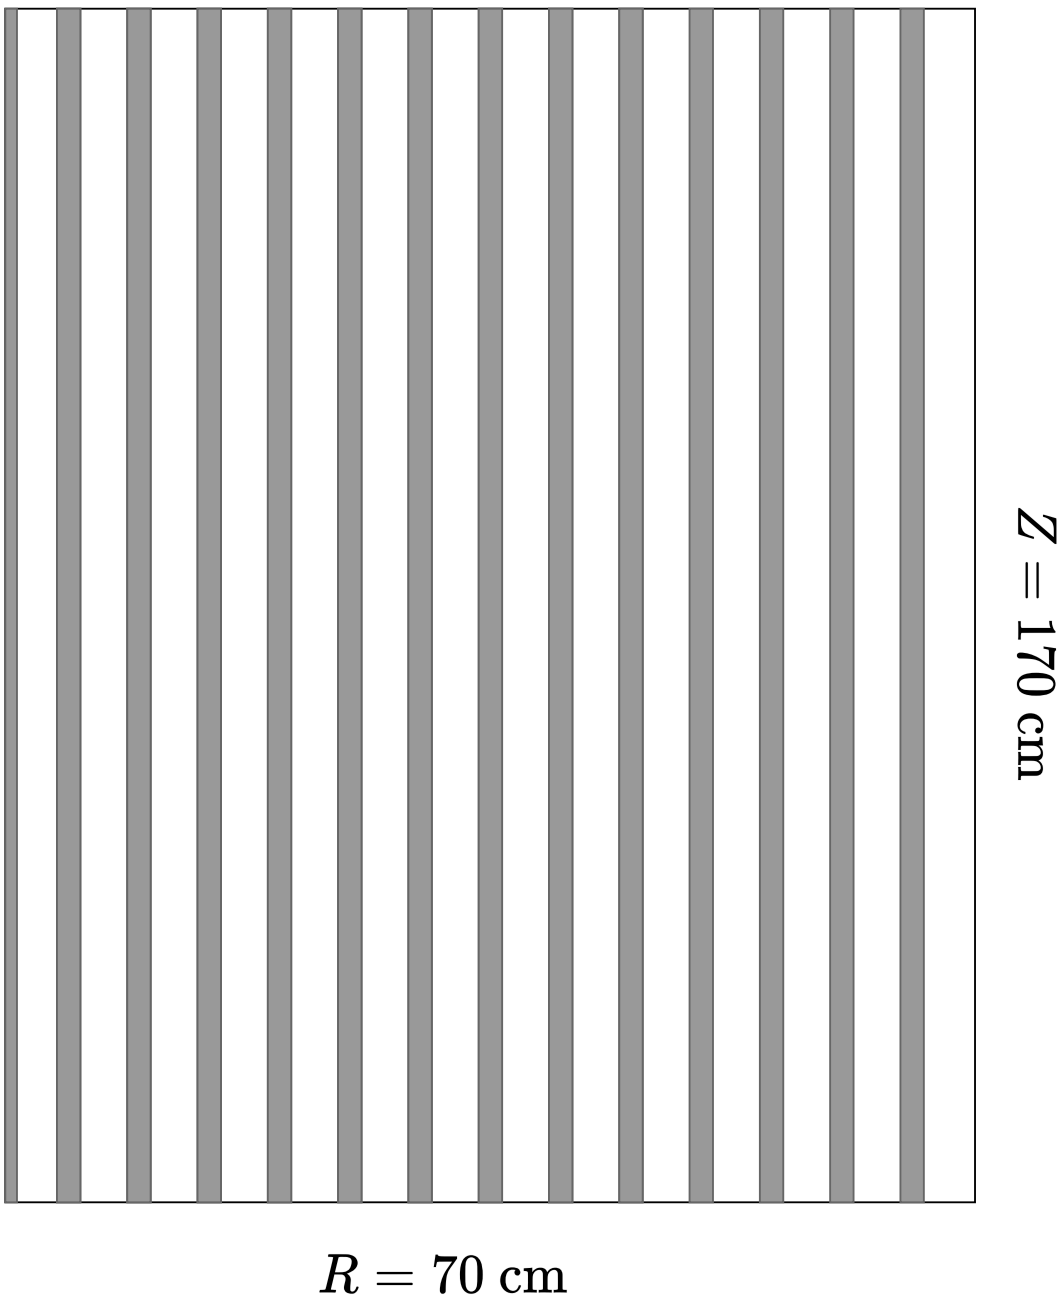
\includegraphics[width=.9\columnwidth]{images/msre-2d}
      \caption{2-D axisymmetric model of the MSRE.}
    \end{figure}
  \end{columns}
\end{frame}

\begin{frame}
  \frametitle{V\&V Study 2: MSRE Pump Start-up \& Coast-Down Transients}
  \begin{block}{\textbf{MSR Phenomena Involved}}
    \begin{itemize}
      \item DNP drift under time-varying flow
      \item Loss of delayed neutrons due to out-of-core DNP decay
    \end{itemize}
  \end{block}
  \begin{block}{\textbf{Aim of the study}}
    Reproduce the reactivity curve of the control rod response with a 2-D axisymmetric model of the
    MSRE in Moltres
  \end{block}
  \begin{block}{\textbf{Objectives}}
    \begin{itemize}
      \item Develop a verification benchmark based on the MSRE pump start-up \& coast-down
        transients that is easily reproducible
      \item Verify Moltres against QuasiMolto in collaboration with Aaron Reynolds
        (formerly at Oregon State University)
      \item Validate Moltres against MSRE experimental data for zero-power pump transients
    \end{itemize}
  \end{block}
\end{frame}

\begin{frame}
  \frametitle{V\&V Study 2: MSRE Pump Start-up \& Coast-Down Transients}
  \begin{columns}
    \column[t]{6.5cm}
    \begin{block}{\textbf{Current Status}}
      \begin{itemize}
        \item Moltres and QuasiMolto simulations (Complete)
        \item Data analysis is in progress (In progress)
        \item Submission for publication (In progress)
      \end{itemize}
    \end{block}
    \begin{block}{\textbf{Extension}}
      Add the upper and lower plena in the 2-D axisymmetric model for improved validation with
      the MSRE experimental data.

      Plena modeling options:
      \begin{enumerate}
        \item Rectangular block with perfect mixing and 1-D flow
        \item Dome-shaped domains with turbulent flow modeling
      \end{enumerate}
    \end{block}
    \column[t]{4.5cm}
    \begin{figure}
      \centering
      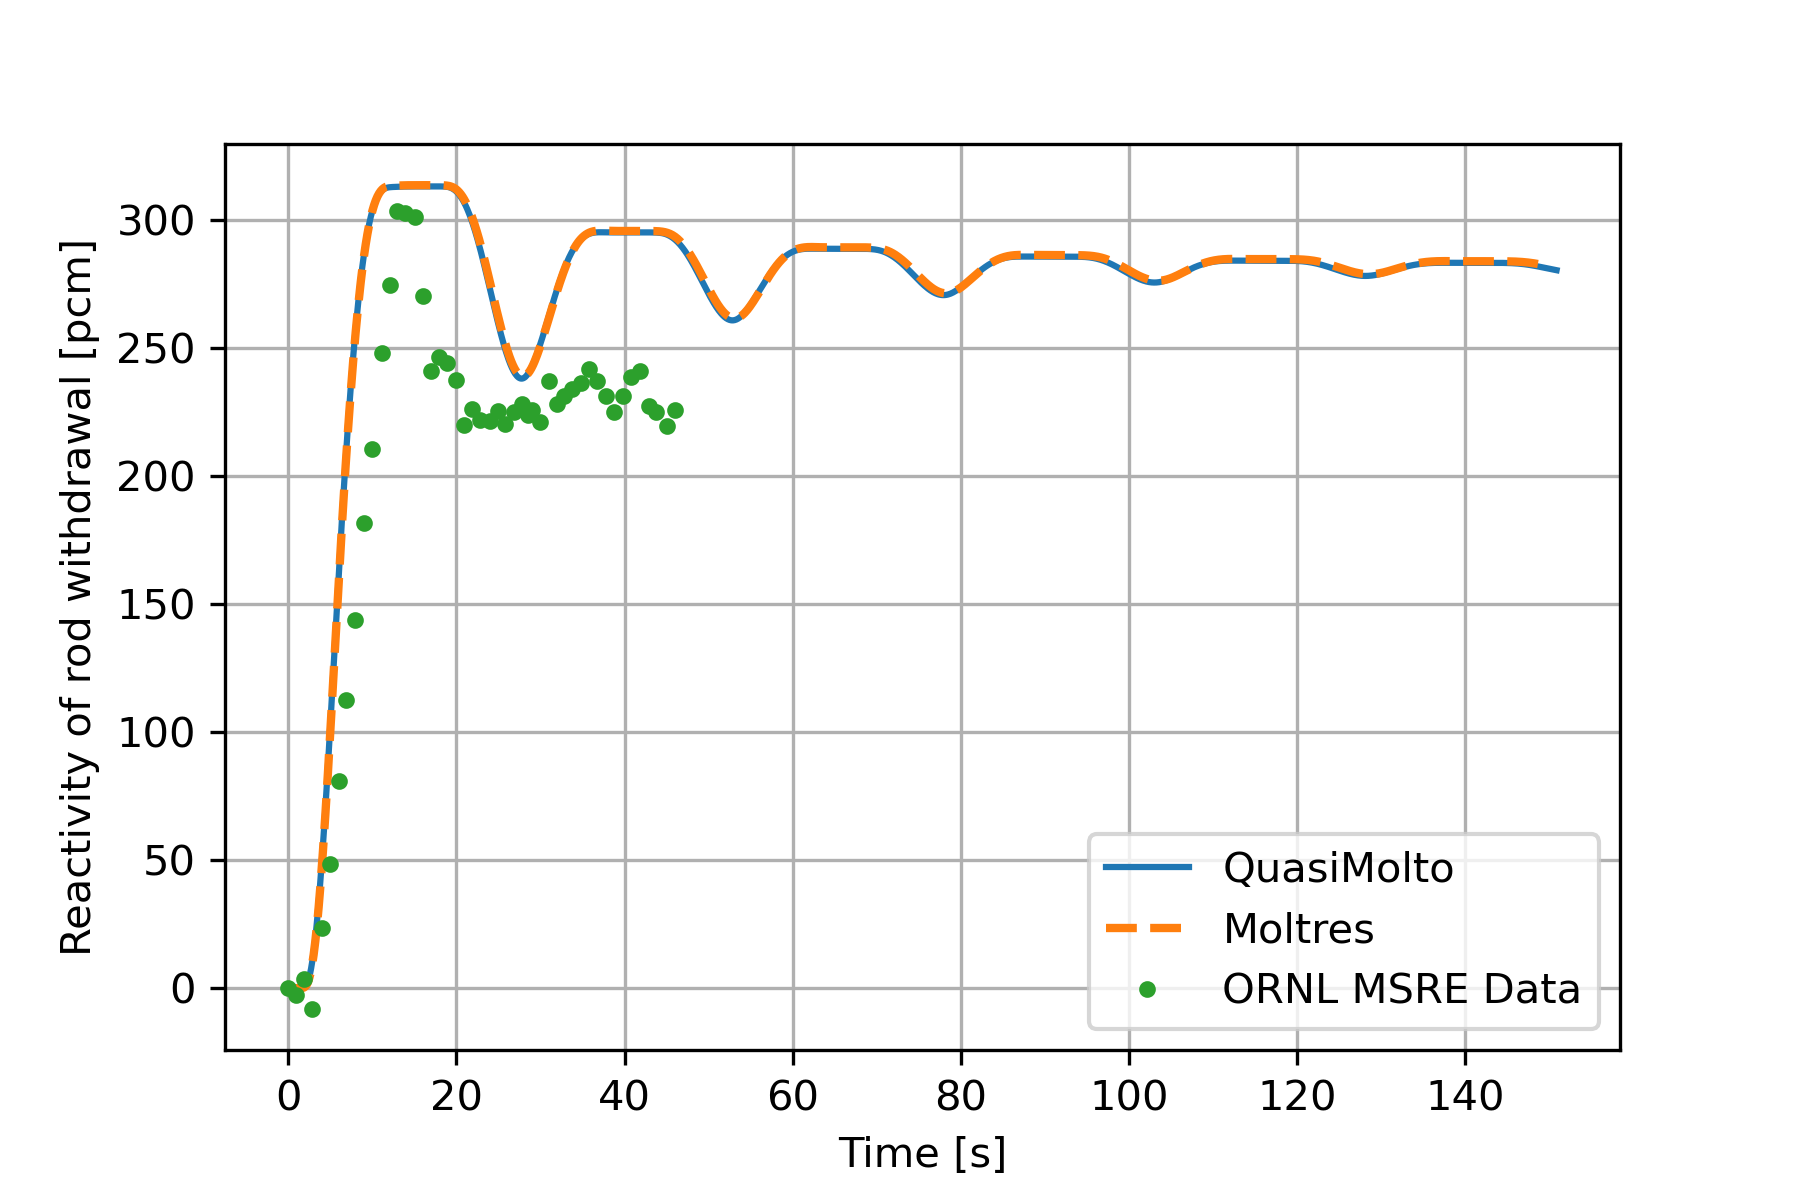
\includegraphics[width=.9\columnwidth]{images/start-up-v2-reactivity}
      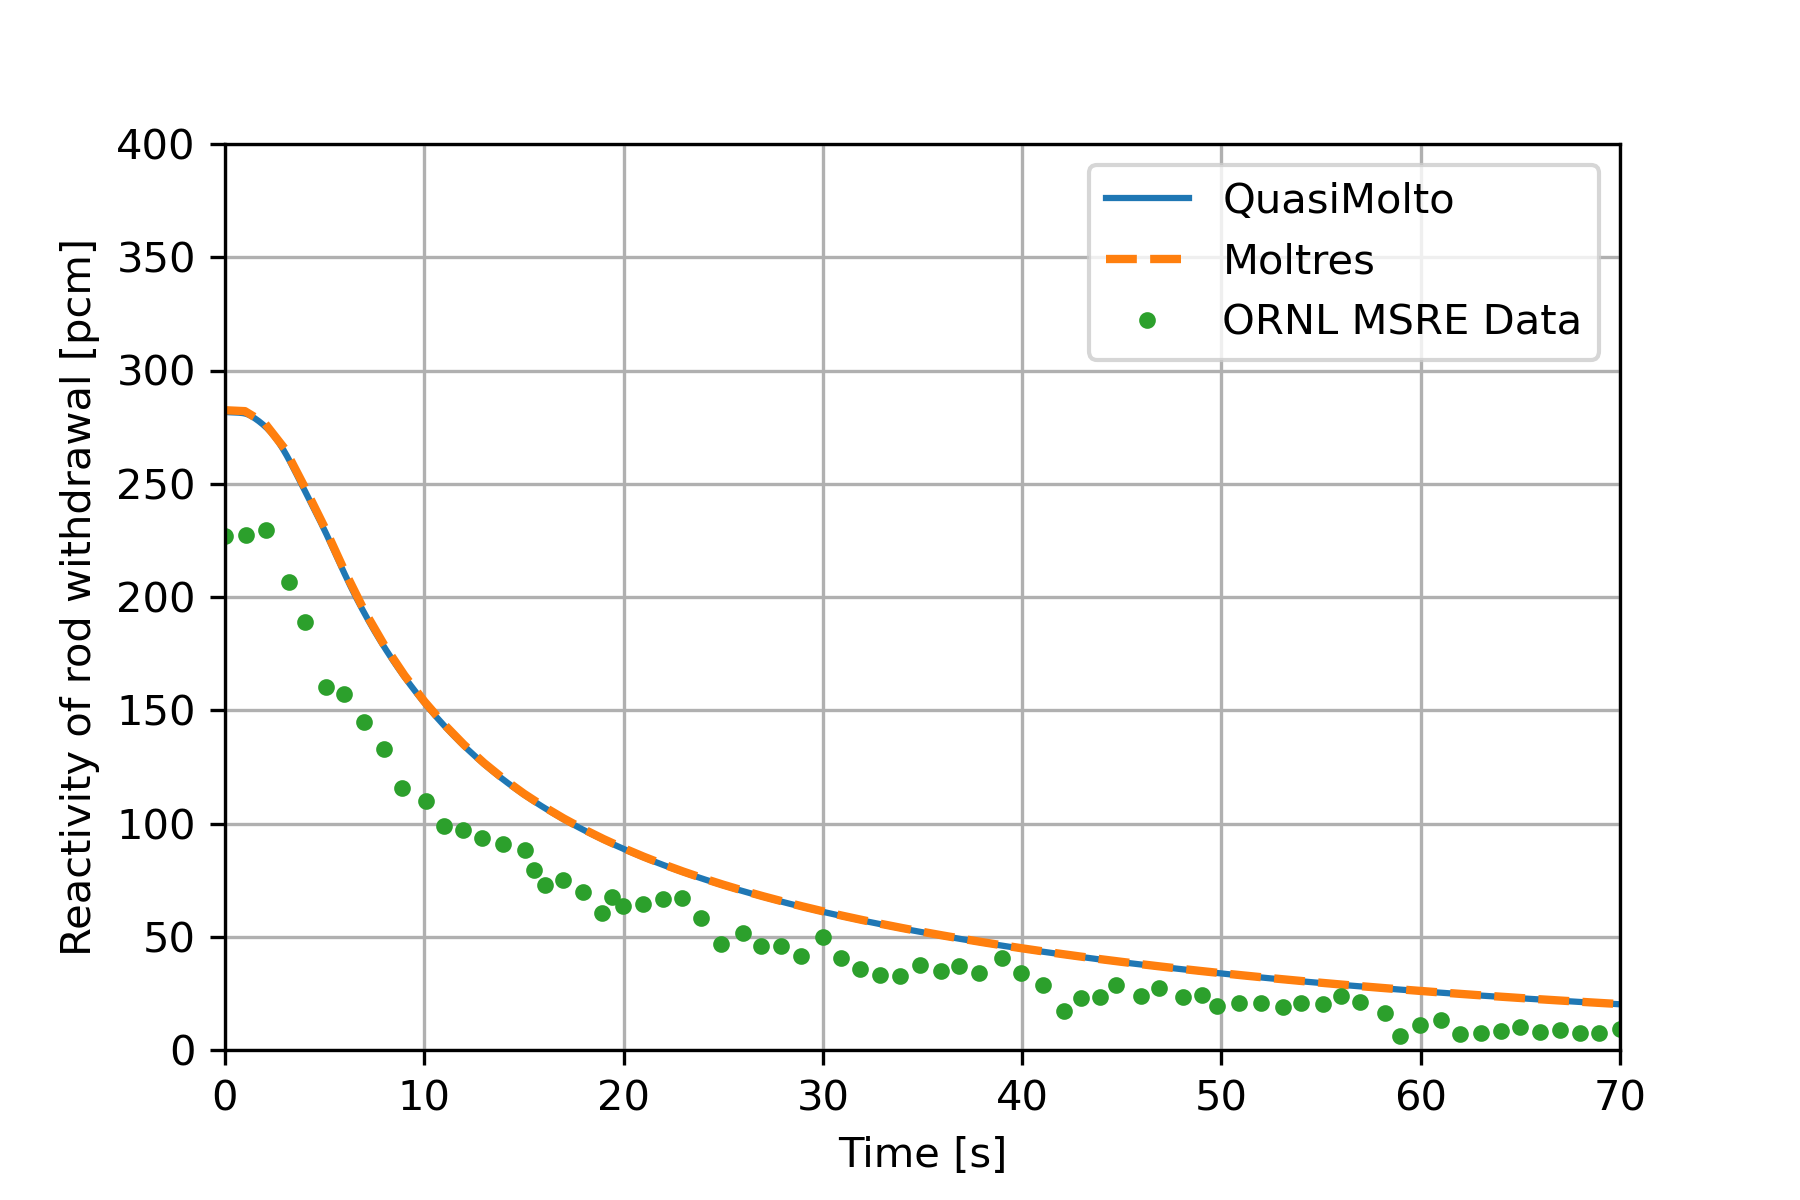
\includegraphics[width=.9\columnwidth]{images/coast-down-v2-reactivity}
      \caption{Reactivity change during the pump start-up (top) and coast-down (bottom)
      transients.}
    \end{figure}
  \end{columns}
\end{frame}

